\documentclass{article}

%% -------------------------------------------------------------------------- %%
%%  Packages
%% -------------------------------------------------------------------------- %%
\usepackage{graphicx}
\usepackage{url}
\usepackage{float}
\usepackage{ragged2e}
\usepackage[margin = 1.25in]{geometry}

\usepackage[backend = bibtex, style = numeric]{biblatex}
\addbibresource{../-1bibliography/bibliography}
\graphicspath{{../-0images/}}


%% -------------------------------------------------------------------------- %%
%%  'ere we go
%% -------------------------------------------------------------------------- %%
\begin{document}

%% -------------------------------------------------------------------------- %%
%%  Cover
%% -------------------------------------------------------------------------- %%
\title{Designing Open Rammed-Earth Systems}
\author{Brian Poirier}
\date{\today}
\maketitle
\clearpage

%% -------------------------------------------------------------------------- %%
%%  TOC
%% -------------------------------------------------------------------------- %%
\tableofcontents
\clearpage


%% -------------------------------------------------------------------------- %%
%%  INTRODUCTION
%% -------------------------------------------------------------------------- %%
\section{INTRODUCTION}

\begin{flushright}
  \small{
  \textit{``The history of building construction can be construed as a narrative of the inertia and momentum of two divergent construction logistics. One mode[, discussed above,] has very minimal historical inertia coupled with great current industrial momentum (the muli-layered assemblies of modernity.) The other has great historical, physical, and thermodynamic inertia that is coupled with minimal industrial momentum in the contemporary building industry/building science industry (more monolithic assemblies and masses). The former follows the short history of the twentieth century ``rationalization" of construction, air-conditioning, factory production, lightweight envelopes, and, more recently, mass customization. The latter is a several-thousand-year history of accumulative knowledge and performance all but forgotten in the interesting yet hubristically selective amnesia of twentieth century architecture."}}\\ --- Kiel Moe. \\ \textit{Convergence}. 2013.
\end{flushright}

``Rammed-earth" refers to an earthen building material formed by a particular mechanical process. Rammed-earth architecture has ancient archaeological, anonymous, and autochthonous roots in China, Africa, Europe, India, the Middle East, and other regions globally \cite{CHRONO}. Observably, rammed-earth forms have been (re)appearing in the U.S. over the past half-century with a frequency and technical gain atypical of earthen construction, especially in the West. Contemporary rammed-earth forms are predominantly connected to academia, professional architectural design, and building science/industry.

Rammed-earth structures have appeared relatively recently on the campuses of M.I.T. (2005), Stanford (2015), and Princeton (2016)\footnote{\url{https://archive.is/5gPbZ} (M.I.T.); \url{https://archive.is/VhpW2} (Stanford); \url{https://archive.is/9SF6K} (Princeton)}. Rammed Earth Works (the designers of Stanford's Windhover Contemplative Center) is one of multiple professional architectural firms to be designing modernized rammed-earth buildings and installations valued in the multimillion-dollar range\footnote{\url{https://archive.is/K853p}}. David Easton, the founder of Rammed Earth Works (1976), also invented PISE (Pneumatically Impacted Rammed Earth) and Watershed Blocks (under a \$750k grant from the N.S.F.); a sprayed application of wet soil-cement and a mechanical system for mass-producing modular soil-cement blocks, respectively. SIREWALL (Structural Insulated Rammed-Earth, B.C., Canada) is a rammed-earth-based building product incorporating an intermediary layer of patented insulation\footnote{\url{https://archive.is/Sf9fu} (PISE); \url{https://archive.is/x3iwg} (Watershed Materials); \url{https://archive.is/s0cHI} (SIREWALL)}. Numerous technical papers concerning rammed-earth's structural and thermal properties have been published globally. A select few include: \textit{Analysis of the hygrothermal functional properties of stabilised rammed-earth materials} by Hall and Allinson. (2009), \textit{Modeling rammed earth wall using discrete element method} by Bui et al. (2015), and \textit{Measured and simulated thermal behaviour in rammed earth houses in a hot-arid climate. Part B: Comfort} by Beckett et al. (2017).

\vspace{5mm}

\underline{Hypothesis:} Along the decades of rammed-earth's previous resurgence in the U.S., at the eco-movements of the 60s and 70s, rammed-earth took on a greater socio-technical momentum while standards, practices, and policies of the building culture remained inert. The result was a form-based function of modern construction---a virtual image of sustainability---reducing, reusing, and recycling a historically function-based form of complexity, persistence, and adaptability. The rammed-earth material \textit{and} method morphed more significantly in forty years than it had in four thousand.

If Doctor E. is right, and we can not solve problems by using the same kind of thinking we used when we created them, then it stands to reason that greater control of contemporary rammed-earth technology is not as much a determinant of sustainability as the model by which rammed-earth forms are conceptualized, codified, communicated, designed, logisticized, and constructed.

\vspace{5mm}

\underline{Objective:} \textbf{Design a system} of design (a coalescing model of models) drawing from contemporary theories and technology, reaching towards the principles and heuristics of the traditional rammed-earth material and method. The model is directed towards a computational system (digital accumulator and distributor of information) capable of organizing two flows:

1. The flow of soil types from deposit to building site (determinants of rammed-earth's embodied energy and building performance).

2. The flow of knowledge between builders (determinant of rammed-earth's standardization and design).


\begin{flushright}
\small{
\textit{``[T]he culture that once was slow-moving, and allowed ample time for adaptation, now changes so rapidly that adaptation cannot keep up with it. No sooner is adjustment of one kind begun than the culture takes a further turn and forces the adjustment in a new direction. No adjustment is ever finished. And the essential condition on the process --- that it should in fact have time to reach its equilibrium --- is violated. This has all actually happened. In our own civilization, the process of adaptation and selection which we have seen at work in the unselfconscious cultures has plainly disappeared."}}\\ --- Christopher Alexander. \\ \textit{Notes on the Synthesis of Form}. 1964.
\end{flushright}


% A precedent similar in its regard for the past is the \textit{Manifesto for responsible architecture}, a one-page document assembled by a collective of architectural collectives and presented at the U.N. Climate Change Conference\in Paris (2015)\footnote{\url{https://web.archive.org/web/20180429205023/https://www.ace-cae.eu/fileadmin/New_Upload/8._Images/News/2015/Manifesto_EN_2.pdf}}. Allegedly, the Manifesto derived from the fossil of Caral, Peru (3,000-1800 B.C.), during a retrospective on the ``high engineering" involved in its structure, from ductwork to urban planning\footnote{\url{http://archive.is/e3wBp}}.



\clearpage

\subsection{The Model is the Message}

Marshall McLuhan noted (\textit{Understanding Media}, 1964) that, with respect to media/technology, the medium is the message. The rammed-earth building medium \textit{qua} pre-modern rammed-earth conveys a natural socio-technical desire for a functional, durable, and economical form of building. Without any positive rammed-earth heritage to draw from, the U.S. has nonetheless considered or adopted rammed-earth construction during energy-sensitive phrases of its history. For instance, in the late-eighteenth century, French architect/builder Fran\c cois Cointereaux presented Thomas Jefferson and America's burgeoning rural economy with a case for rammed-earth architecture. Encoded in a copy of \textit{Ecole d'architecture rurale} (Paris, 1790-91), Cointereaux believed that if America adopted ``the economical building art of the ancients, perfected and made more universal," She would incur a great physiocratic power. Jefferson reacted indifferently, in a letter to William Short, ``how far it may offer benefit here superior to the methods of the country, founded in the actual circumstances of the country as to the combined costs of labour \& materials, and the circumstances of durability comfort \& appearance, must be the result of calculation."\footnote{\url{http://archive.is/yWexi} (Cointereaux to Jefferson); \url{http://archive.is/ozqQv} (Jefferson to Short)}

Rammed-earth later appeared in \textit{Popular Mechanics (Vol. 41, No. 2, 1924)} and \textit{The Farmers Bulletin  (No. 1500, 1926)}, endorsed as a frugal, Do-It-Yourself building method. During the Great Depression, rammed-earth briefly held the attention of the New Deal-era Resettlement Administration as an economical building alternative fit for an over-abundance of available labor. Around the 1960s and 1970s, rammed-earth attracted marginal interest from the environmental movements, following the global recognition of troubling anthropogenic effects on the biosphere and building's major role aside this phenomenon \cite{GARDENDALE}. Speculatively, following this last wave of rammed-earth building in the U.S., although the material would continue in some form, the D.I.Y.ness was lost to the momentum/inertia of building practices.

In a gross linearization of history, it would appear that a growing field around ``ecodevelopment" in the 1960s/1970s effectively reintroduced rammed-earth building for the first time into a technologically dependent world aware of the consequences of (in binary terms) developmentalist and zero-growth economic strategies\footnote{\url{http://archive.is/sOf7w}}. Hypothetically, at this shearing of [simply] technological positivity and technological negativity, building societies retrofit rammed-earth into a model through which cake could be had and also eaten. On one hand, the tried method would remain a symbol of building sustainability. On the other, seemingly innocuous technical changes to rammed-earth's composition and construction would modernize the material-method, ensuring marketability, scalability, standardization, and security.

Rammed-earth v2.0 manifested as ``soil-cement", also known as ``cement stabilized rammed-earth." Over time, it was layered with modernizing assemblages of mechanization, pre-fabrication, insulation, transportation, seal-ification, svelte-ification and modularization. An early code of practice was \textit{Soil-Cement: Its Use in Building}, distributed by the U.N. Department of Economic and Social Affairs in 1964.

\begin{flushright}
\small{
\textit{``The use of simple compacted soil (natural earth) as a building material dates from time immemorial, and it can be said that ever since, and down to the present day, the method of building houses with earth has been used, because of its constructive qualities. Yet, despite its} good insulating and resistant properties [author's emphasis], \textit{there are limitations to the use of earth owing to its lack of strength and its vulnerability to moisture and the erosive effects of external agents. Provided that natural soil possesses a combination of certain characteristics, however, it can be subjected to the process known as `stabilization'. The effect of adding a stabilizing agent like Portland cement, for instance, is not only to enhance its best qualities but to impart to it other properties which soil alone does not possess."}}\\ --- Augusto A. Enteiche \\ \textit{Soil-Cement: Its Use in Building}. 1964.
\end{flushright}


\begin{flushright}
\small{
\textit{
``Contemporary stabilized rammed earth (SRE) draws upon traditional rammed earth (RE) methods and materials, often incorporating reinforcing steel and rigid insulation, enhancing the structural and energy performance of the walls while satisfying building codes. SRE structures are typically engineered by licensed Structural Engineers using the Concrete Building Code or the Masonry Building Code."}} \\ --- Bly Windstorm and Arno Schmidt. \\ \textit{A Report of Contemporary Rammed-Earth Construction and Research in North America}. 2013.
\end{flushright}


Generally, the above quotes represent modern/contemporary models concerning rammed-earth's function as a building material, physically and also with regard to their respective building cultures. Endemic to both rationalizations is [what is now seen to be \cite{MOECONVERGENCE}] a destructive reduction of vital qualities (or non-qualities) of rammed-earth building, e.g. ``resistant properties" and questionably ``[enhanced]" energy performance.

McLuhan's wisdom remains, the cement-stabilized rammed-earth medium conveys the message that, as Bruce Sterling noted (\textit{Shaping Things}, 2005), the model is the message. Rammed-earth ceases to exist as an unselfconscious technology of sustenance and increasingly becomes defined by complicated logistics, stylistic preferences, and virtual references. This is to say that contemporary rammed-earth \textit{in rem} does not necessarily possess the property of sustainability. Instead, the historical ability of rammed-earth to sustain itself, its settlers, its ecosystem, and the biosphere at large is a phenomenon emerging from the inanimate and animate collectives involved in rammed-earth building, i.e. its model.

\clearpage

%% -------------------------------------------------------------------------- %%
%%  AN ARCHITECTURAL THEORY ABOUT THERMODYNAMICS AND A THERMODYNAMICAL THEORY ABOUT ARCHITECTURES
%% -------------------------------------------------------------------------- %%
\section{AN ARCHITECTURAL THEORY ABOUT THERMODYNAMICS AND A THERMODYNAMICAL THEORY ABOUT ARCHITECTURES}
\subsection{An Architectural Agenda for Energy}

Architect/builder/author/professor Kiel Moe has authored a number of texts and a number of buildings in and around the past decade that cogently and convergently embody a novel theory about building(s) and energy. ``An Architectural Agenda for Energy", the subtitle of \textit{Convergence}, describes a ``more totalizing" conjunction of building systems with the subtle yet opportunistic complexities of energy typically siloed off to engineering and applied science. In this way, the Agenda predicates healthier building dynamics (more durable and effective flows of matter/energy), in turn, predicating healthier inhabitants (re: Sick Building Syndrome, Building Related Illness) and healthier ecosystems (holistic environmental accounting) \cite{MOECONVERGENCE}. The Agenda and its network of references form an ideal system with which rammed-earth's contemporary presence may be bridged to its sustainable history. This section is dedicated to fitting rammed-earth design and building further into the Agenda, hopefully with minimal gain in conceptual entropy from Professor Moe's work. At once, the Agenda reflects latent, useful properties of the rammed-earth material and method as well as the terrifically complicated, complicating mega-structure of building rammed-earth currently finds itself in.

Professor Moe explicitly references rammed-earth at least twice. Once, in the Building Lecture Series at the University of Virginia\footnote{\url{http://archive.is/u9TKf}}, in the context of rammed-earth as a thermally massive building material. Capillary to this vein, Professor Moe discusses the material quantities thermal effusivity (\textit{e}) and thermal diffusivity ($\alpha$) contributing to a more wholesome understanding of building materials as thermally transient, interactive, qualitative systems rather than scientifically ideal systems forever operating in the steady-state mode. Second, Professor Moe references rammed-earth as a case study in \textit{Convergence}: the Granturismo Earth and Stone project in southern Portugal. Initially a reforestation initiative funded by the European Union, the project entailed ten rammed-earth and stone structures in the inner Algarve region suited for tourism and recreation. In this remote area, the locally-sourced property of rammed-earth proved to be critical for design, construction, economic, and ecological reasons. Furthermore, the Algarve does possess a positive heritage in rammed-earth building and Granturismo was an opportunity to ``[make] the history of the Algarve material culture apparent while [the material selection reinvests] in the labor and skill connected to that material." \cite{MOECONVERGENCE}

In the next three subsections, rammed-earth codes, performance, and energetics are drawn around the Architectural Agenda for Energy. The ultimate motivation for doing so is founded in the fact that the Agenda values the historical inertia of rammed-earth with its contemporary potential in a profoundly integrated manner. Ostensibly, no other theory of building draws across disciplinary boundaries (engineering, physics, architecture, ecology, history, economics. . .) nor across scales (``From the Molecular to the Territorial"\footnote{\url{http://archive.is/7lXIB}}) so applicably.

At a high level, the socio-technical, building codification is regarded as a great challenge and a great opportunity to preserve traditional rammed-earth. At an intermediate level, material and thermal performances of rammed-earth are considered in light of standard building envelopes. At a third level, the quantum and the global simultaneously, quantities and qualities of energy are considered as they pertain to the design and construction of rammed-earth buildings.



\subsubsection{Rammed-Earth Codes}



\subsubsection{Rammed-Earth Performance}



\subsubsection{Rammed-Earth Energetics}


% \begin{flushright}
\small{
\textit{
``Many historical and modernized systems of building with unstabilized earth exist around the globe, and comprise the housing for a large percentage of humanity. In many cases, multiple examples can be found of extant structures with many centuries of useful service life, none of which have been designed by engineers. The durability, utility, and appeal of earthen construction is thus established, and historical systems in particular express designs generally well adapted to local climate and conditions."}} \\ --- ASTM International. \\ \textit{Standard Guide for Design of Earthen Wall Building Systems : Appendix X1 : Empirical Design and Minimum Detailing Requirements for Earthen Structures}. 2010.
\end{flushright}

A side effect of rammed-earth's relative dormancy in the U.S. is a lack of centralized, homogenized research data (when compared to concrete or steel, for instance) or a unified science for guiding rammed-earth construction from wild soil to building performance and eventual deterioration. Historically, the rammed-earth building process has been guided by the immediate intuition and somatosensory judgements of experienced builders \cite{RAMMEDEARTHHOUSE}. In contemporary rammed-earth building, the scientific viewport is of great importance. Essential considerations range from the seismic behavior of geographic regions to the chemical behavior of clay particles.

Both of these construction logistics are evidenced across an array of modern building guides, codes and standards. In the empirical sense, formal guides such as ASTM E2392/E2392M (Appendix X1) appear to be relatively liberal with the techniques and quantities involved in rammed-earth construction. Granted a single-story building in a seismically low-risk area, methods such as the ``Ball Test" and the ``Roll Test" provide approximate values for design and construction. In the modern scientio-industrial sense, codes such as the New Mexico Earthen Building Materials Code demand stabilization on the order of six percent by weight of Portland cement and laboratory testing on a set of samples prepared from the site\footnote{\url{https://archive.is/2wkiN}}. Joe Dahmen (principal investigator/designer for the rammed-earth wall at M.I.T.) reported, in discussion with a Tuscon-based rammed-earth builder, ``builders often increase the amount of Portland cement to double the amount specified to avoid a shortage of cement in the mix, which is measured by approximate means in the field.\footnote{\url{https://archive.li/WP2Uf}}"

The constitutional complexity of rammed-earth is a challenge and an opportunity. It is a challenge because the emergent performance of a rammed-earth is determined by an ensemble of microscopic particles and resultant pore structure, fuzzy pre-factors of construction such as water content, compaction energy, the configuration of the structure, local topology, hydrology, and weather/climate patters, to name only a few factors.

This complexity may also be one of rammed-earth's great assets. By keeping track of a finite representation of these parameters in a centralized, visible, and open format, an outward-facing standard may evolve not simply around ensuring an arbitrary value of mechanical strength, but also around the customization of performance per local geology and geography.

This is a case for empirical science in rammed-earth building and standardization, mainly but not exclusively opposed to analytical models and ``top-down" standards which lack the capability to express this complexity without years of abstracting laboratory research and much mathematical rigidity. Whether empirical data is somehow integrated or plainly recorded and made accessible, it is a quick and transparent mode of science that has the potential to become more detailed and also adapting in time with new data. The artistic aspect of rammed-earth has not prohibited experimentation with tempers such as lime, straw, or chaff \cite{RAMMEDEARTHHOUSE}. An empirically open standard is able to facilitate and propagate new practices, while a closed, prescribed standard prohibits timely adaptability.

A notable link between the geographic and the geological is the steady accumulation of pedological information over time. Saliently, the U.S. Soil Survey began in 1899 as an endeavor based in the utility of knowledge about soil for e.g. agricultural and constructional purposes. Since, the database has been digitized and covers more than ninety-five percent of the nation's counties \footnote{\url{http://archive.li/hD4CZ}}. Of note is SoilGrids\footnote{\url{http://archive.is/l07N3}}, a machine learning-based pedological model drawing from several independent sources and projecting results at a spatial resolution of 250 meters.

Queryable soil properties of the Soil Survey include: percent clay, percent sand, percent silt, linear extensibility, plasticity index, AASHTO group classification, and Unified soil classification.

\begin{figure}[H]
  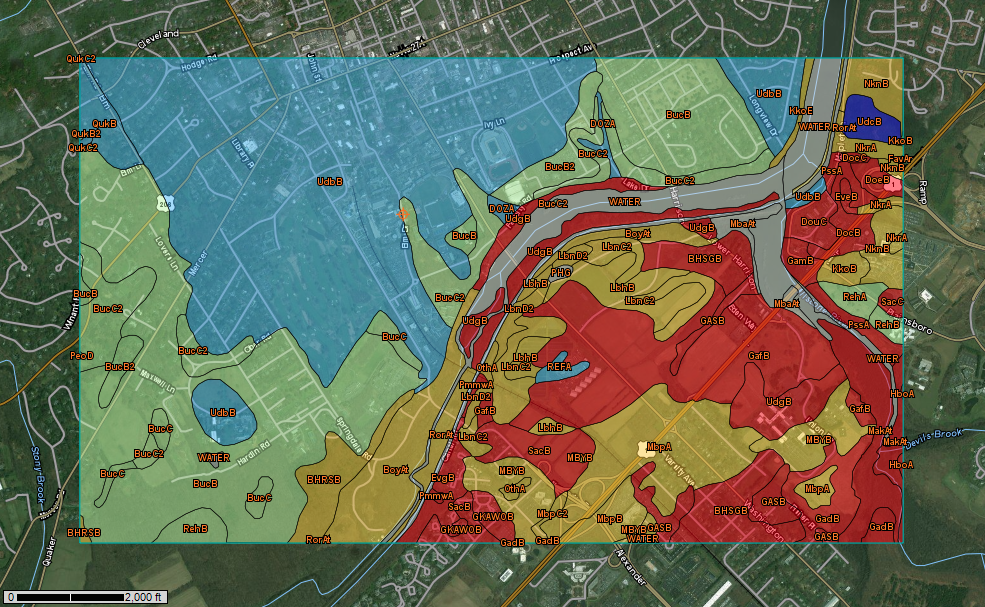
\includegraphics[scale=0.45]{wss1}

  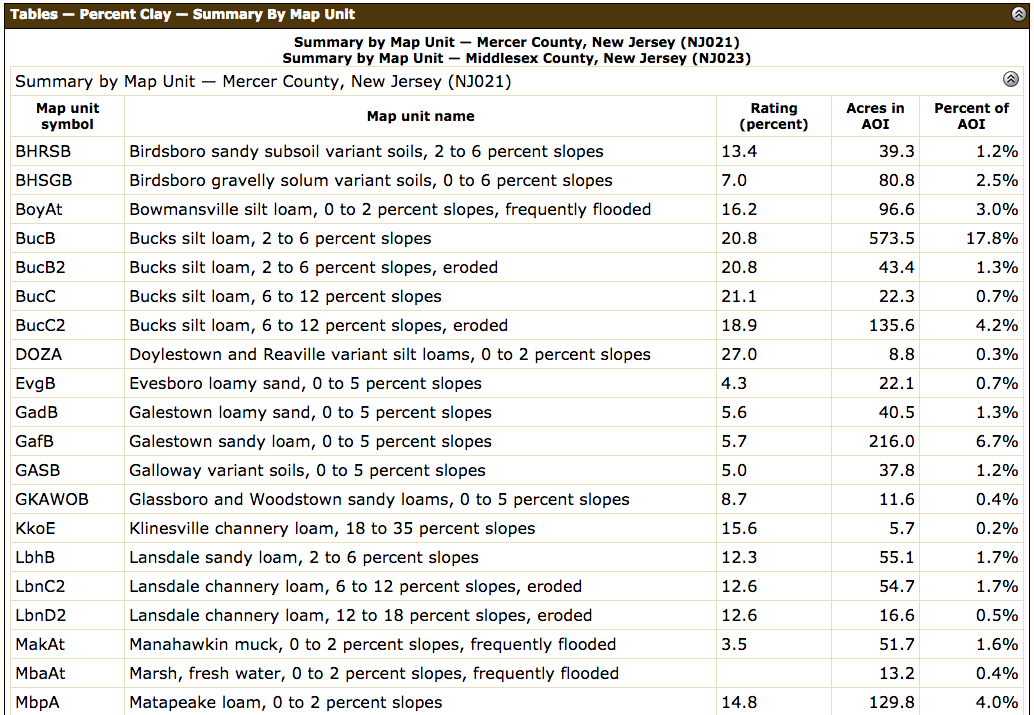
\includegraphics[scale=0.43]{wss2}
\end{figure}






\begin{flushright}
\small{
\textit{``What holds for the pyramids and the ant hills holds for all our logistics and manufacturing operations."}}
\end{flushright}

\vspace{5mm}

\begin{flushright}
\small{
\textit{``The pyramid and the quarry grow at the same time. If the pyramid is a positive architecture (y $<$ 0), the quarry is its negative. Such positive-negative pairs are everywhere in history and geography, even though modern advances in transportation technology tend to obscure them" }}\\ --- Adrian Bejan \\ \textit{Advanced Engineering Thermodynamics, Third Edition}. 2006.
\end{flushright}

A main consequence of readily available geo-spatial information is the optimization of soil convergence as an area-to-point flow. Adrian Bejan describes this phenomenon in pyramid and ant hill construction, wherein the location and the shape of pyramids and ant hills around the world are predicted by applying a principle of least work \cite{FLOWFOSSIL}.

Saliently, this connection between ancient principle and modern technology stands to offer a previously unseen level of accountability for rammed-earth building. Designers are able to openly access (Web Soil Survey:SQL, SoilGrids:JSON) soil information local to their site, determine where and not where soil may be accessed, and predicate rammed-earth material composition around the local soilscape and climate. Emergy-oriented design decisions can be made between, for instance, adding two percent more cement, or transporting additional clay from twenty miles away.



%% -------------------------------------------------------------------------- %%
%%  BOURNE-AGAIN SHELLS: COMPUTATION IN BUILDING
%% -------------------------------------------------------------------------- %%


%% -------------------------------------------------------------------------- %%
%%  DESIGNED SYSTEM
%% -------------------------------------------------------------------------- %%



% \nocite{*}
\printbibliography

\end{document}



%% Notes
% value of an air gap or extended thickness in RE wall vs. insulation
% diffusivity and effusivity
